\section{The Adaptation Layer}
\label{sec:adaptation_layer}

The second layer of the AdaptUI architecture is the Adaptation Layer. After the
processes performed by the Modelling Layer, the Adaptation Layer aims to lead the
dynamic adaptation of the elements presented in the user interface. It is formed
by two different modules: The Adaptation Engine, which purpose is to adapt the
currently interface shown by the device, and the Adaptation Polisher, which aims
the refinement of the user interface basing its task in several usability metrics.


\subsection{The Adaptation Engine}
\label{sec:adaptation_engine}

After the storage of the domain knowledge in the AdaptUIOnt ontology by the
Semantic Modeller, several rules are triggered. These rules are grouped in three
different subsets: the pre-adaptation rules, the adaptation rules and the post-adaptation
rules. More concretely, the adaptation rules subset is the one which modifies
the knowledge represented by the \textit{Adaptation} class in the AdaptUIOnt
ontology.

Once these rules have been executed the Adaptation Engine requests these results
to the \textit{Adaptation} class. Then, it launches several methods to dynamically
change the aspect of the current user interface. These methods basically redraw
and refresh the different components shown in the current activity, sharing
their new characteristics to the rest of activities. 

Listing~\ref{lst:redraw} shows an example of how several views are redrawn.
First, the elements that are part of the activity (i.e., buttons and textviews)
are initialized (similarly to other applications). Next, several methods regarding
the adaptation are called. The \textit{redrawViews()} method takes into account
the user's configured profile through the Capabilities Collector and adapts the
components of the activity accordingly. Every activity overwrites this method
(and others), as they extend from a parent abstract class called
\textit{AbstractActivity}. This class mainly manages the services initialization
(e.g., TextToSpeech) and the ontology. 
% Listing~\ref{lst:abstract_activity} shows
% part of the AdaptUI source code where the ontology is initialized.


\inputminted[linenos=true, fontsize=\footnotesize, frame=lines]{java}{4_system_architecture/redraw.java}
\captionof{listing}{Example of the creation and adaptation of an activity. In this case 
the example is centred in the adaptation of a button.\label{lst:redraw}}

% \inputminted[linenos=true, fontsize=\footnotesize, frame=lines]{java}{4_system_architecture/abstract_activity.java}
% \captionof{listing}{The AbstractActivity class ontology related methods.\label{lst:abstract_activity}}

Listing~\ref{lst:store_in_ontology} shows a piece of source code where the developer
uses the \ac{owl}-\ac{api} to store the user profile in the AdaptUIOnt model. 
% The methods called in this example are part of the Turambar framework~\citep{david_ausin_probabilistic_2014}. 
% This framework provides a high-level \ac{api} for managing the \ac{owl}-\ac{api}.

\inputminted[linenos=true, fontsize=\footnotesize, frame=lines]{java}{4_system_architecture/store_in_ontology.java}
\captionof{listing}{Inserting values in the corresponding classes of the AdaptUIOnt 
ontology.\label{lst:store_in_ontology}}


Finally, Figure~\ref{fig:adaptation_differences} shows two activities with the
same user interface. The difference is that the activity on the left is showing
the default user interface defined in the activity's layout. On the contrary,
the activity on the right shows adapted components in its interface.

\begin{figure}[H]
\centering
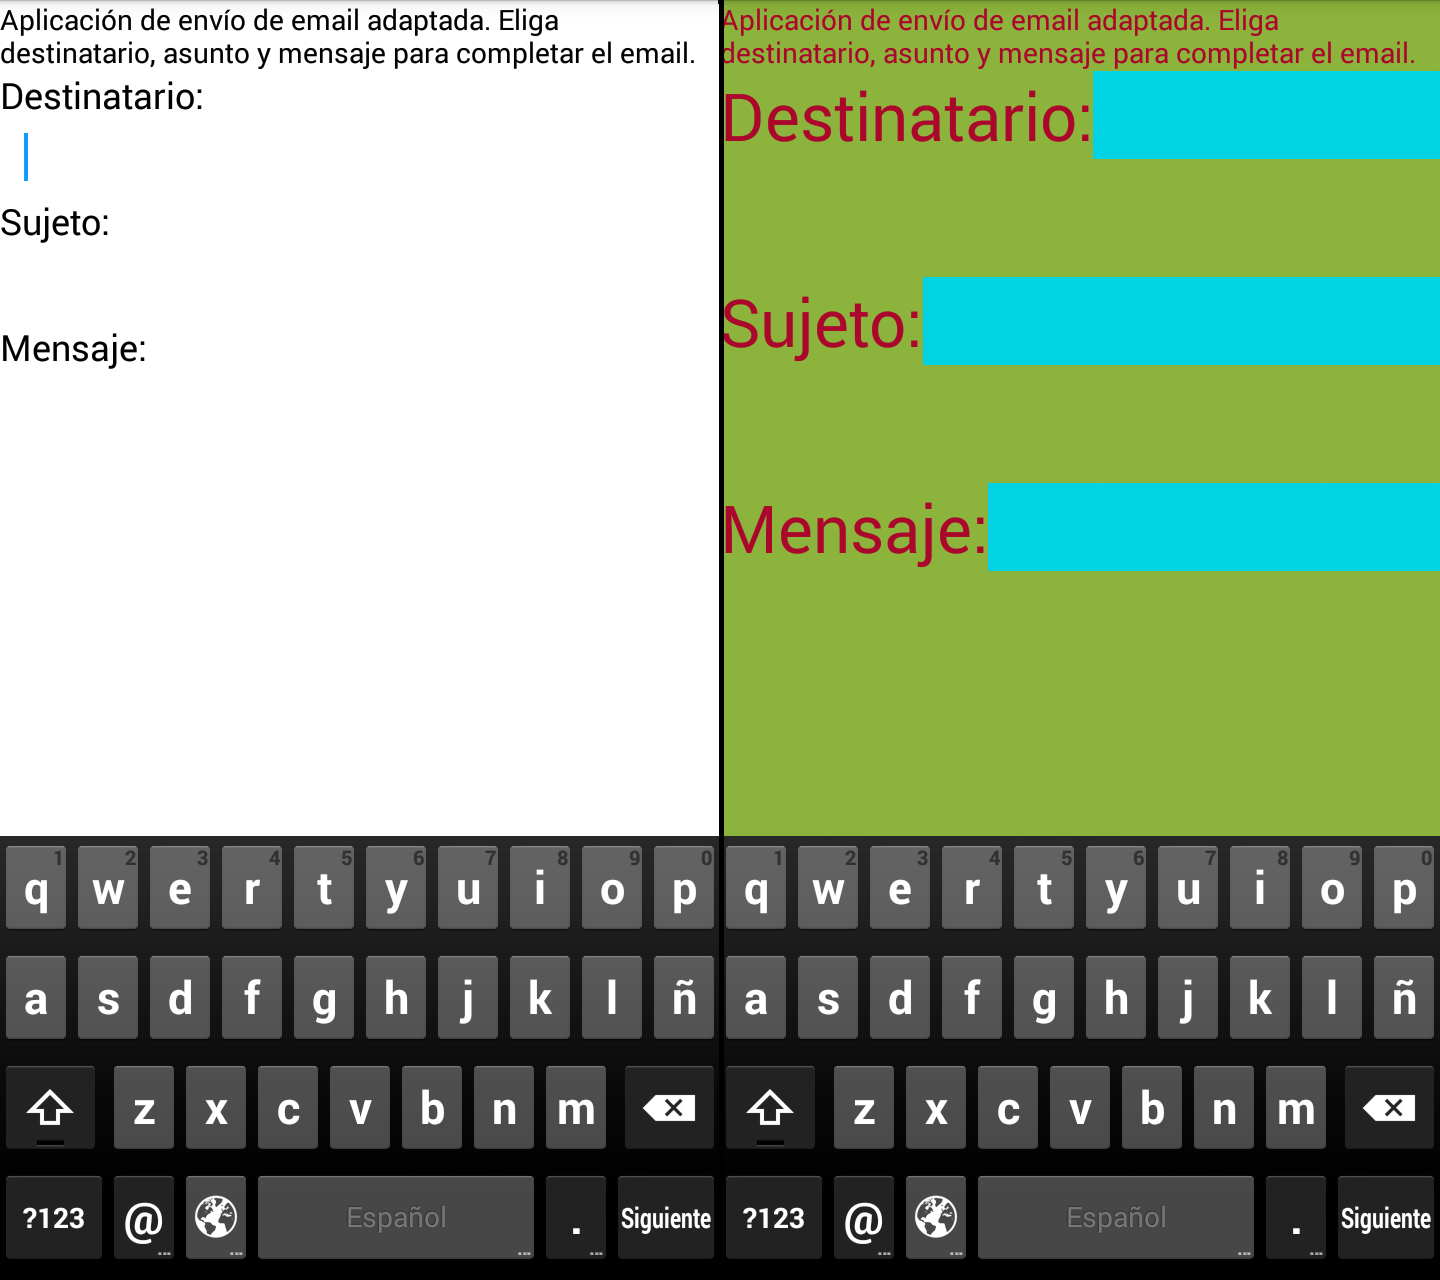
\includegraphics[width=0.65\textwidth]{adaptation_differences.png}
\caption{User interface adaptation performed by the Adaptation Engine. On the
left, a default activity with no adaptation. On the right, the same activity
after the adaptation process. As is shown, the colours sets and sizes of each
component of the adapted user interface are different from the non adapted one.}
\label{fig:adaptation_differences}
\end{figure}


\subsection{The Adaptation Polisher}
\label{sec:adaptation_polisher}

Although the adaptations for the user follow the instructions detailed by him/her,
there is still the possibility that the Adaptation Engine's results lead to a
unsuccessful interaction/adaptation. One of the main reasons for this is that
the classification of the model, considering the context aspects, is just an
approximation of the reality. For example, considering that between 1,000 \ac{lx} and
25,000 \ac{lx} the reasoner determines that the ontology value for the luminance
is \textit{daylight}, the difference might be significant in real scenarios
(see Table~\ref{tbl:luminance}). In other words, the user might easily interact
with a 1,000 \ac{lx} context light but tediously in a 24,999 \ac{lx} light environment. In
order to tackle this problem, there are two possible solutions: to consider
an extensive set of classification rules including more possible situations (e.g.,
dividing the luminance table into more categories), or to design a specific
module which evaluates the user interaction results: the Adaptation Polisher.

The first case is difficult to implement. Nevertheless, AdaptUI provides an \ac{api}
which aims to help in this issue allowing developers to create and modify the
ontology knowledge. This means that it is possible to try to model every tiny
context variation to capture different context characteristics and adapt the user
interface accordingly. However, this is not practical, and AdaptUI covers the
second case with the Adaptation Polisher. Therefore developers do not have to
model these small variations in the environment.

The Adaptation Polisher is a software module, part of the Adaptation Layer, which
monitors the effectiveness and responsiveness of the adapted interfaces. Collecting
different usability and productivity metrics of the interaction carried out by the
user, this module is able to make small but specific adaptations to improve
the ongoing interaction. This module has been designed considering the relative
user efficiency productivity metrics. These metrics compare the efficiency of the
user compared to an expert. But it has no sense to compare the user with others
in AdaptUI. The system cannot generalize and apply adaptations based on other
users' preferences. To solve this, in AdaptUI we propose to maintain a base
adaptation, which thanks to the Adaptation Polisher and its interaction results
will be improved. Consequently, an interaction model is built for each adaptation.
Therefore, we can determine the efficiency of the user when he/she is manipulating
an adaptation made by the system by comparing the last adaptation to the previous
one.

% AdaptUI keeps an interaction model of the user (as an expert) stored in the
% ontology. Once an adaptation is made, the Adaptation Polisher monitors the user
% interaction and then checks the stored model with the new generated one. Next,
% the post-adaptation rules are triggered.


\subsubsection{The Usability Metrics}
\label{sec:usability_metrics}
For this module, several usability metrics have been studied and implemented.
These metrics are classified into two different groups: effectiveness metrics
and productivity metrics.

Table~\ref{tbl:effectiveness_metrics} and Table~\ref{tbl:productivity_metrics}
detail the usability metrics implemented in AdaptUI. The following information
is given for each metric in the cited tables:

\begin{enumerate}[label=\alph*)]
  \item Purpose of the metric: Expresses the main goal of the current metric.
  \item Measurement, formula and data element computations: Provide the formulas
  to compute the current metric and the meaning of the used data elements.
  \item Interpretation of the measured value: Details the range and preferred values.
  \item Metric scale type: Provides the type of scale used by the current metrics.
  The possible scale types are: Nominal, Ordinal, Interval, Ratio and Absolute
  scale.
  \item Measure type: Provides the type of the measure. The possible measure
  types are: Size, Time and Count.
\end{enumerate}

In the original \ac{iso}document~\citep{ISOIEC9126} there are 4 extra columns that
have not been included in Table~\ref{tbl:effectiveness_metrics} and
Table~\ref{tbl:productivity_metrics}. This is because the values for each metric
under these columns are the same:

\begin{enumerate}[label=\alph*)]
  \item Method of application: Provides an outline of the application. 
  
  \item Input to measurement: Details the source of data used in the measurement.
  In this case there are two inputs that each metric shares: Operation (test) 
  report and User monitoring record.
  
  \item Reference: Identifies software life cycle processes where the metric is
  applicable. There are three processes that each metric shares: 6.5 Validation,
  5.3 Qualification testing and 5.4 Operation.
  
  \item Target audience: Identifies the user(s) of the measurement results. Again,
  the metrics share User and Human interface designer as their audiences.
\end{enumerate}


\myparagraph{Effectiveness Metrics}
\label{sec:effectiveness_metrics}
Effectiveness metrics, as detailed in the \ac{iso}/\ac{iec} 9126-4~\citep{ISOIEC9126},
evaluate whether the current task achieves a specific goal considering the accuracy
and completeness of the corresponding task. These metrics are shown in
Table~\ref{tbl:effectiveness_metrics}.


% \begin{landscape}
\begin{table}
  \caption{The effectiveness metrics used in the Adaptation Polisher, as it appears in~\citep{ISOIEC9126}.}
 \label{tbl:effectiveness_metrics}
\footnotesize
\centering
 \begin{tabular}{l l l l l l}
  \hline 
\textbf{Metric}	& \textbf{Purpose of }	& \textbf{Measurement,}		& \textbf{Interpretation }	& \textbf{Metric}	& \textbf{Measure} 	\\
\textbf{name}   & \textbf{the metrics}	& \textbf{formula and data}	& \textbf{of measured }		& \textbf{scale}   	& \textbf{type}		\\
		& 			& \textbf{element compu-}	& \textbf{value}		& \textbf{type}					\\
		& 			& \textbf{tations}												\\
\hline
Task  		& To measure the 	& $M1=|1-\Sigma A_{i}|$		&  $0\leq M1 \leq 1$		& \textemdash 		& $A=$ proportion 	\\
effectiveness	& proportion of the  	& 				&				& 			& 			\\
		& goals of the task	& $A_{i}=$ proportional  	& The closer to			& 			& 			\\
		& achieved 		& value of each 		& 1.0 the better.		& 			& 			\\
		& correctly.		& missing or incorrect 		& 				& 			& 			\\
		& 			& component in the 	\\
		& 			& task output		\\
\hline	  
Task  		& To measure the 	& $X=A/B$			& $0\leq X \leq 1$    		& Ratio 		& $A=$ Count 		\\
completion 	& proportion of  	& 				& 				& 			& $B=$ Count		\\
		& the task that 	& $A=$ number of 		& The closer to			& 			& $X=$ Count/Count	\\
		& is completed.		& tasks completed		& 1.0 the better.		& 			& 			\\  
		& 			& $B=$ total number of		& 				& 			& 			\\
		& 			& tasks attempted	\\
\hline
Error  		& To measure the 	& $X=A/T$			& $0\leq X$  	  		& Absolute 		& $A=$ Count 		\\
frequency 	& frequency of 		& 				& 				& 			&~			\\
		& errors.		& $A=$ number of 		& The closer to			& 			&~			\\
		& 			& errors made by the 		& 0 the better.			& 			&~			\\  
		&			& user			\\
		& 			& $T=$ time or number 		& 				& 			& 			\\
		& 			& of tasks 		\\
\hline

\end{tabular}
\end{table}

% \end{landscape}


\myparagraph{Productivity Metrics}
\label{sec:productivity_metrics}
Productivity metrics evaluate the resources consumed by the users in relation
to the effectiveness achieved in the current task~\citep{ISOIEC9126}. These 
metrics are shown in Table~\ref{tbl:productivity_metrics}.


% \begin{landscape}
\begin{table}
  \caption{The productivity metrics used in the Adaptation Polisher, as it appears in~\citep{ISOIEC9126}.}
 \label{tbl:productivity_metrics}
\footnotesize
\centering
  \begin{tabular}{l l l l l l}
  \hline 
\textbf{Metric}	& \textbf{Purpose of }	& \textbf{Measurement,}		& \textbf{Interpretation }	& \textbf{Metric}	& \textbf{Measure} 	\\
\textbf{name}   & \textbf{the metrics}	& \textbf{formula and data}	& \textbf{of measured }		& \textbf{scale}   	& \textbf{type}		\\
		& 			& \textbf{element compu-}	& \textbf{value}		& \textbf{type}					\\
		& 			& \textbf{tations}												\\
\hline
Task  		& To measure the 	& $X=Ta$			& $0\leq X$			& Interval 		& $T=$ Time	 	\\
time		& required time to	& 				&				& 			& 			\\
		& complete the task.	& $Ta=$ Task time		& The closer to			& 			& 			\\
		& 		 	& 				& 1.0 the better.		& 			& 			\\
\hline	  
Task  		& To measure how 	& $X=M1/T$			& $0\leq X \leq 1$    		& \textemdash 		& $T=$ Time		\\
efficiency 	& efficient the 	& 				& 				& 			& $X=$ proportion/	\\
		& users are.		& $M1=$ task 			& The larger the		& 			& time			\\
		&			& effectiveness			& better.			& 			& 			\\
		& 			& $T=$ task time		& 				& 			& 			\\  
\hline
Economic  	& To measure the	& $X=M1/C$			& $0\leq X$  	  		& \textemdash 		& $C=$ Value 		\\
productivity 	& cost-effectiveness	& 				& 				& 			&~			\\
		& of the user.		& $M1=$ task 			& The larger the		& 			&~			\\
		& 			& effectiveness			& better.			& 			&~			\\
		& 			& $C=$ total cost 		& 				& 			&~			\\ 
		& 			& of the tasks													\\

\hline
Productive	& To measure the  	& $X=Ta/Tb$			& $0\leq X \leq 1$  		& Absolute 		& $Ta=$ Time 		\\
proportion 	& proportion of 	& 				& 				& 			& $Tb=$ Time		\\
		& time the user 	& $Ta=$ productive 		& The closer to 		& 			& $X=$ Time/		\\
		& is performing		& time = task time - 		& 1.0 the better.		& 			& Time			\\  
		& productive actions.	& help time - error 		& 				& 			& 			\\
		& 			& time - search time \\
		& 			& $Tb=$ task time \\
\hline
Relative user  	& To measure the  	& Relative user			& $0\leq X \leq 1$  		& Absolute 		& $C=$ proportion/ 	\\
efficiency 	& efficiency of 	& efficiency			& 				& 			& time			\\
		& the user compared 	& $X=A/B$			&				& 			&~			\\
		& to an expert.		& 				& 				& 			& 			\\
		& 			& $A=$ ordinary 		& The closer to			& 			&~			\\  
		&			& user's task 			& 1.0 the better.		& 			& 			\\
		&			& efficiency 	\\
		& 			& $B=$ expert 			& 				& 			& 			\\
		& 			& user's task 			& 				& 			& 			\\
		& 			& efficiency	\\
\hline

\end{tabular}
\end{table}

% \end{landscape}


\subsubsection{Adaptation Polisher Scenario}
\label{sec:adaptation_polisher_scenario}

In the following lines a scenario describing step by step the actions performed
by the Adaptation Polisher is presented. Table~\ref{tbl:polisher_adaptation} 
shows the inferred adaptation for the user, context and device characteristics 
described in Table~\ref{tbl:polisher_scenario}.

\begin{table}
 \caption{Scenario situation summary.}
 \label{tbl:polisher_scenario}
 \footnotesize
 \centering
\begin{tabular}{l l}
  \hline 
				& \textbf{Scenario}		\\
  \hline
  User \\
  \qquad - Personal data 	& David, 23 years old, Spanish 	\\
  \qquad - Activity	 	& - 				\\
  \qquad - Known disabilities 	& - 				\\
% 				& Hearing loss 			\\
%   \hline
  Context \\
  \qquad - Location 		& Relative: Vitoria, Spain  	\\
				& 				\\
  \qquad - Time			& 06:30 			\\
  \qquad - Brightness		& 600 \ac{lx} 			\\
  \qquad - Temperature		& -5 ºC 			\\
%   \hline
  Device 			& Motorola Moto G 	 	\\
% 				& 				\\	
  \hline
  Task				& Send an email			\\
  \hline
\end{tabular}
\end{table}

\begin{table}
 \caption{Final adaptation for the presented scenario.}
 \label{tbl:polisher_adaptation}
 \footnotesize
 \centering
\begin{tabular}{l l}
  \hline 
%     \multicolumn{2}{c}{\textbf{Scenario 2}}	\\
    \textbf{Adaptation} 	& \textbf{Value}\\
    \hline
%     \textit{hasBrightness}	& ???		\\
    \textit{hasColourSet}	& -		\\
    \textit{hasViewSize}	& 10		\\
    \textit{hasResponse}	& vibration	\\
%     \textit{hasColourSet}	& Colour blindness 	\\
%     \textit{hasViewSize}	& 20 			\\
%     \textit{hasInput}		& Voice and haptic	\\
    \textit{hasInput}		& Default	\\
    \textit{hasOutput}		& Visual and audio\\
    \textit{hasVolume}		& 5 		\\
  \hline
\end{tabular}
\end{table}

As Table~\ref{tbl:polisher_scenario} shows, David does not suffer from any
disability. Nevertheless, the context situation presents characteristics that
might trouble David during the interaction process. The cold temperature and the
lack of sufficient light requires a user interface adaptation. Thus, AdaptUI
increases the device's brightness and the views' sizes. 
Figure~\ref{fig:polisher_scenario} illustrates the differences between the 
default user interface (left) and the adapted one (right).

\begin{figure}
\centering
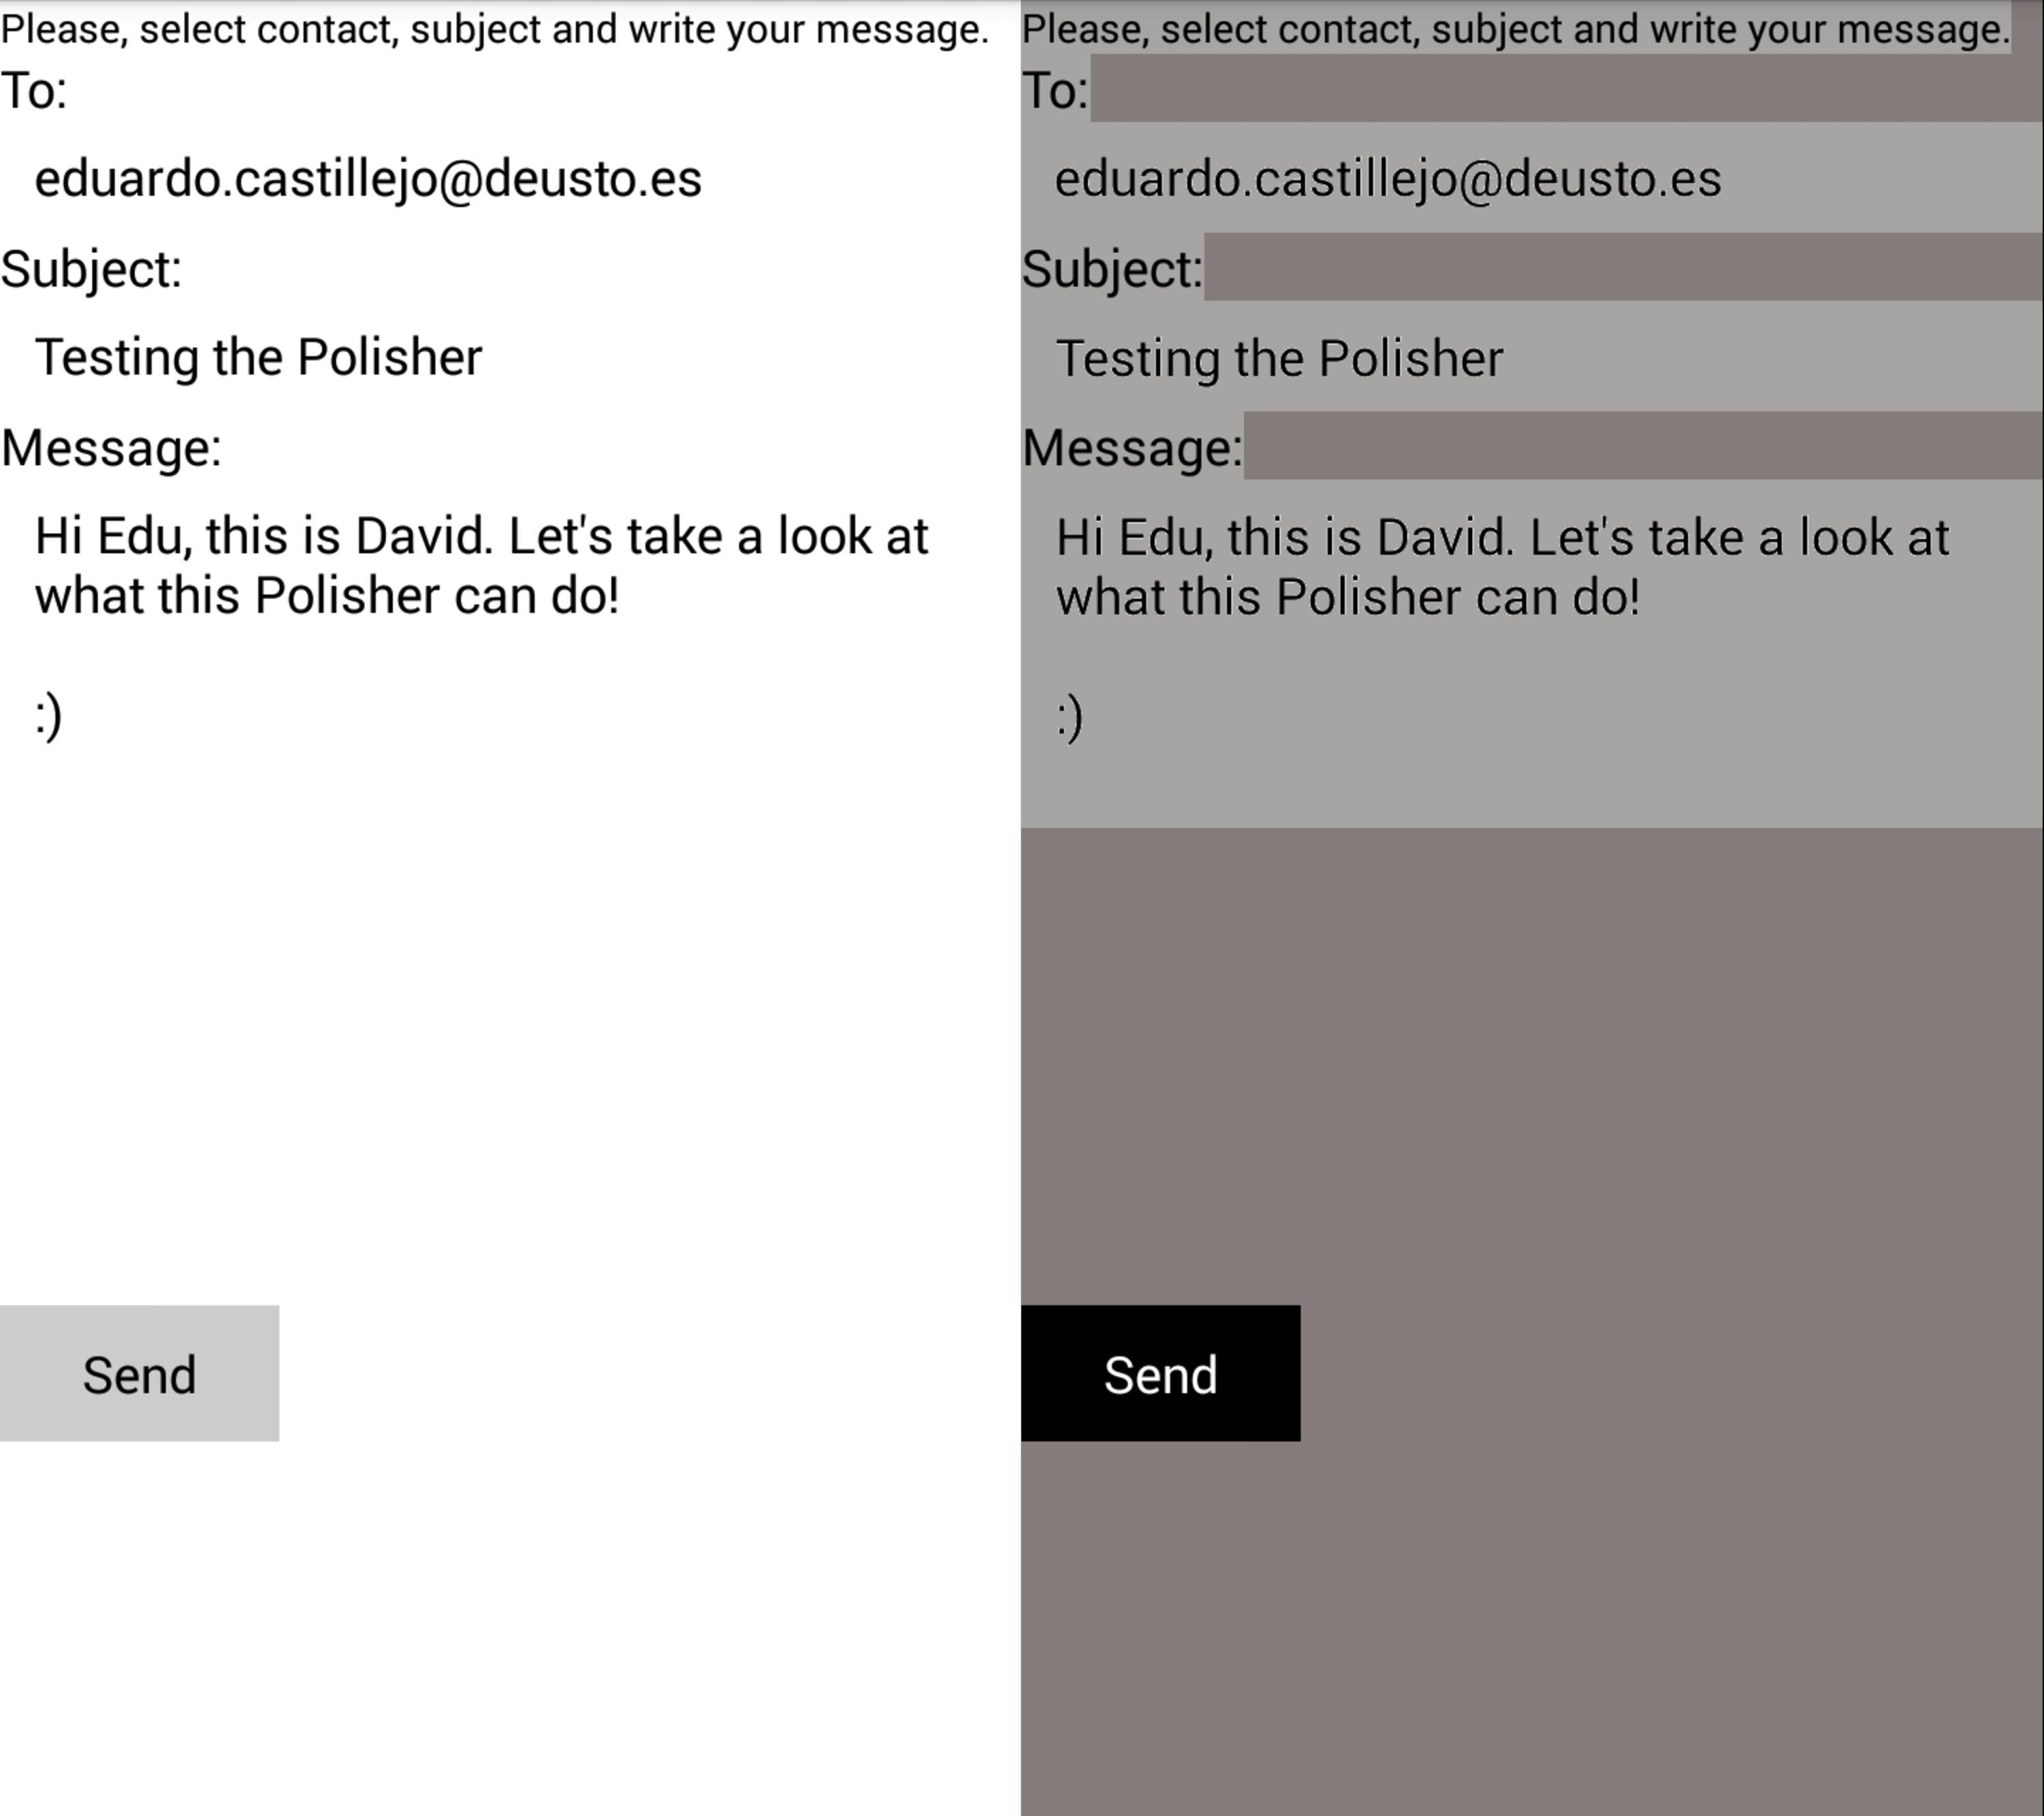
\includegraphics[width=0.65\textwidth]{polisher_scenario.pdf}
\caption{User interface adaptation performed by the Adaptation Engine. On the
left, the default version, without adaptations. On the right, the same 
application adapted by AdaptUI.}
\label{fig:polisher_scenario}
\end{figure}

Thus, David uses his device through the adapted user interface. At this point,
the corresponding interaction model is built by the Adaptation Layer, collecting
the usability metrics shown in Section~\ref{sec:usability_metrics} (see 
Table~\ref{tbl:effectiveness_metrics} and Table~\ref{tbl:productivity_metrics}).
Table~\ref{tbl:model_comparison} shows the used metrics and the computed values
for both the default and the adapted interaction models.

\begin{table}
 \caption{The interaction model computed by the Adaptation Layer. Time ($T$) has
 been measured in seconds.}
 \label{tbl:model_comparison}
 \footnotesize
 \centering
\begin{tabular}{l l l}
  \hline 
  \textbf{Metric} 	& \textbf{Value for the default}& \textbf{Value for the adapted}\\
			& \textbf{interaction model} 	& \textbf{interaction model}	\\
  \hline
  Task effectiveness	& 0.7				& 0.350	\\
  ($M1=|1-\Sigma A_{i}|$)\\
  Task completion	& 1				& 0	\\
  ($X=A/B$)\\
  Error frequency 	& 0.2				& 0.562	\\	%3/15, 18/32 
  ($X=A/T$)\\
  \hline
  Task time		& 15				& 32	\\
  ($X=Ta$)\\
  Task efficiency 	& 0.046				& 0.010	\\
  ($X=M1/T$)\\
%   Productive proportion\\
%   ($X=Ta/Tb$)\\
  Relative user efficiency & 1.0			& 0.5	\\
  ($X=A/B$)\\
  \hline
\end{tabular}
\end{table}

As is shown in Table~\ref{tbl:model_comparison}, the resulting adapted user 
interface provided by AdaptUI does not improve the interaction of the user.
The required time for performing the same task (sending an email) is 32 seconds,
while by default David uses 15 seconds approximately. Thus, the user interface
does not fit the user needs. 

Once the interaction model has been built, the Adaptation Polisher checks the
usability rules set. As detailed in Section~\ref{sec:adaptation_polisher}, these
rules trigger the polisher rules if certain usability ranges are exceeded.
Equation~\ref{ec:usability_rule} shows a usability rule checking the relative
user efficiency of the interaction model.

\footnotesize
\begin{equation} \label{ec:usability_rule}
  \begin{align*} 
  UserAux(?user) ∧ Productivity(?productivity) ∧ Polisher(?polisher) ∧\\ 
  userAuxHasProductivityMetrics(?user, ?productivity) ∧ \\
  hasRelativeEfficiency(?productivity, ?efficiency) ∧ \\
  lessThanOrEqual(?efficiency, 0.5) ∧ \\
  \Rightarrow \\
  launchPolisherRules(?polisher, true)
  \end{align*}
\end{equation}
\normalsize

On the other hand, Equation~\ref{ec:polisher_rule} is triggered by 
Equation~\ref{ec:usability_rule}. In the consequent of this rule there is 
a value of $1.10$. This value means that the size of the views presented in the
previous adapted version of the user interface should be increased in a $10\%$
Hence, the next rule polishes the adapted user
interface.

\footnotesize
\begin{equation} \label{ec:polisher_rule}
  \begin{align*} 
  Polisher(?polisher) ∧ launchPolisherRules(?polisher, true) ∧\\
  UserAux(?user) ∧ userAuxHasEffectivenessMetrics(?user, ?effectiveness) ∧ \\
  effectivenessMetricHasErrorFreequency(?effectiveness, ?freq?) ∧\\
  greaterThan(?freq, 0.5)\\
  \Rightarrow \\
  setViewSize(1.10)
  \end{align*}
\end{equation}
\normalsize

Thus, the resulting polished user interface is shown in Figure~\ref{fig:polisher_4}.

\begin{figure}
\centering
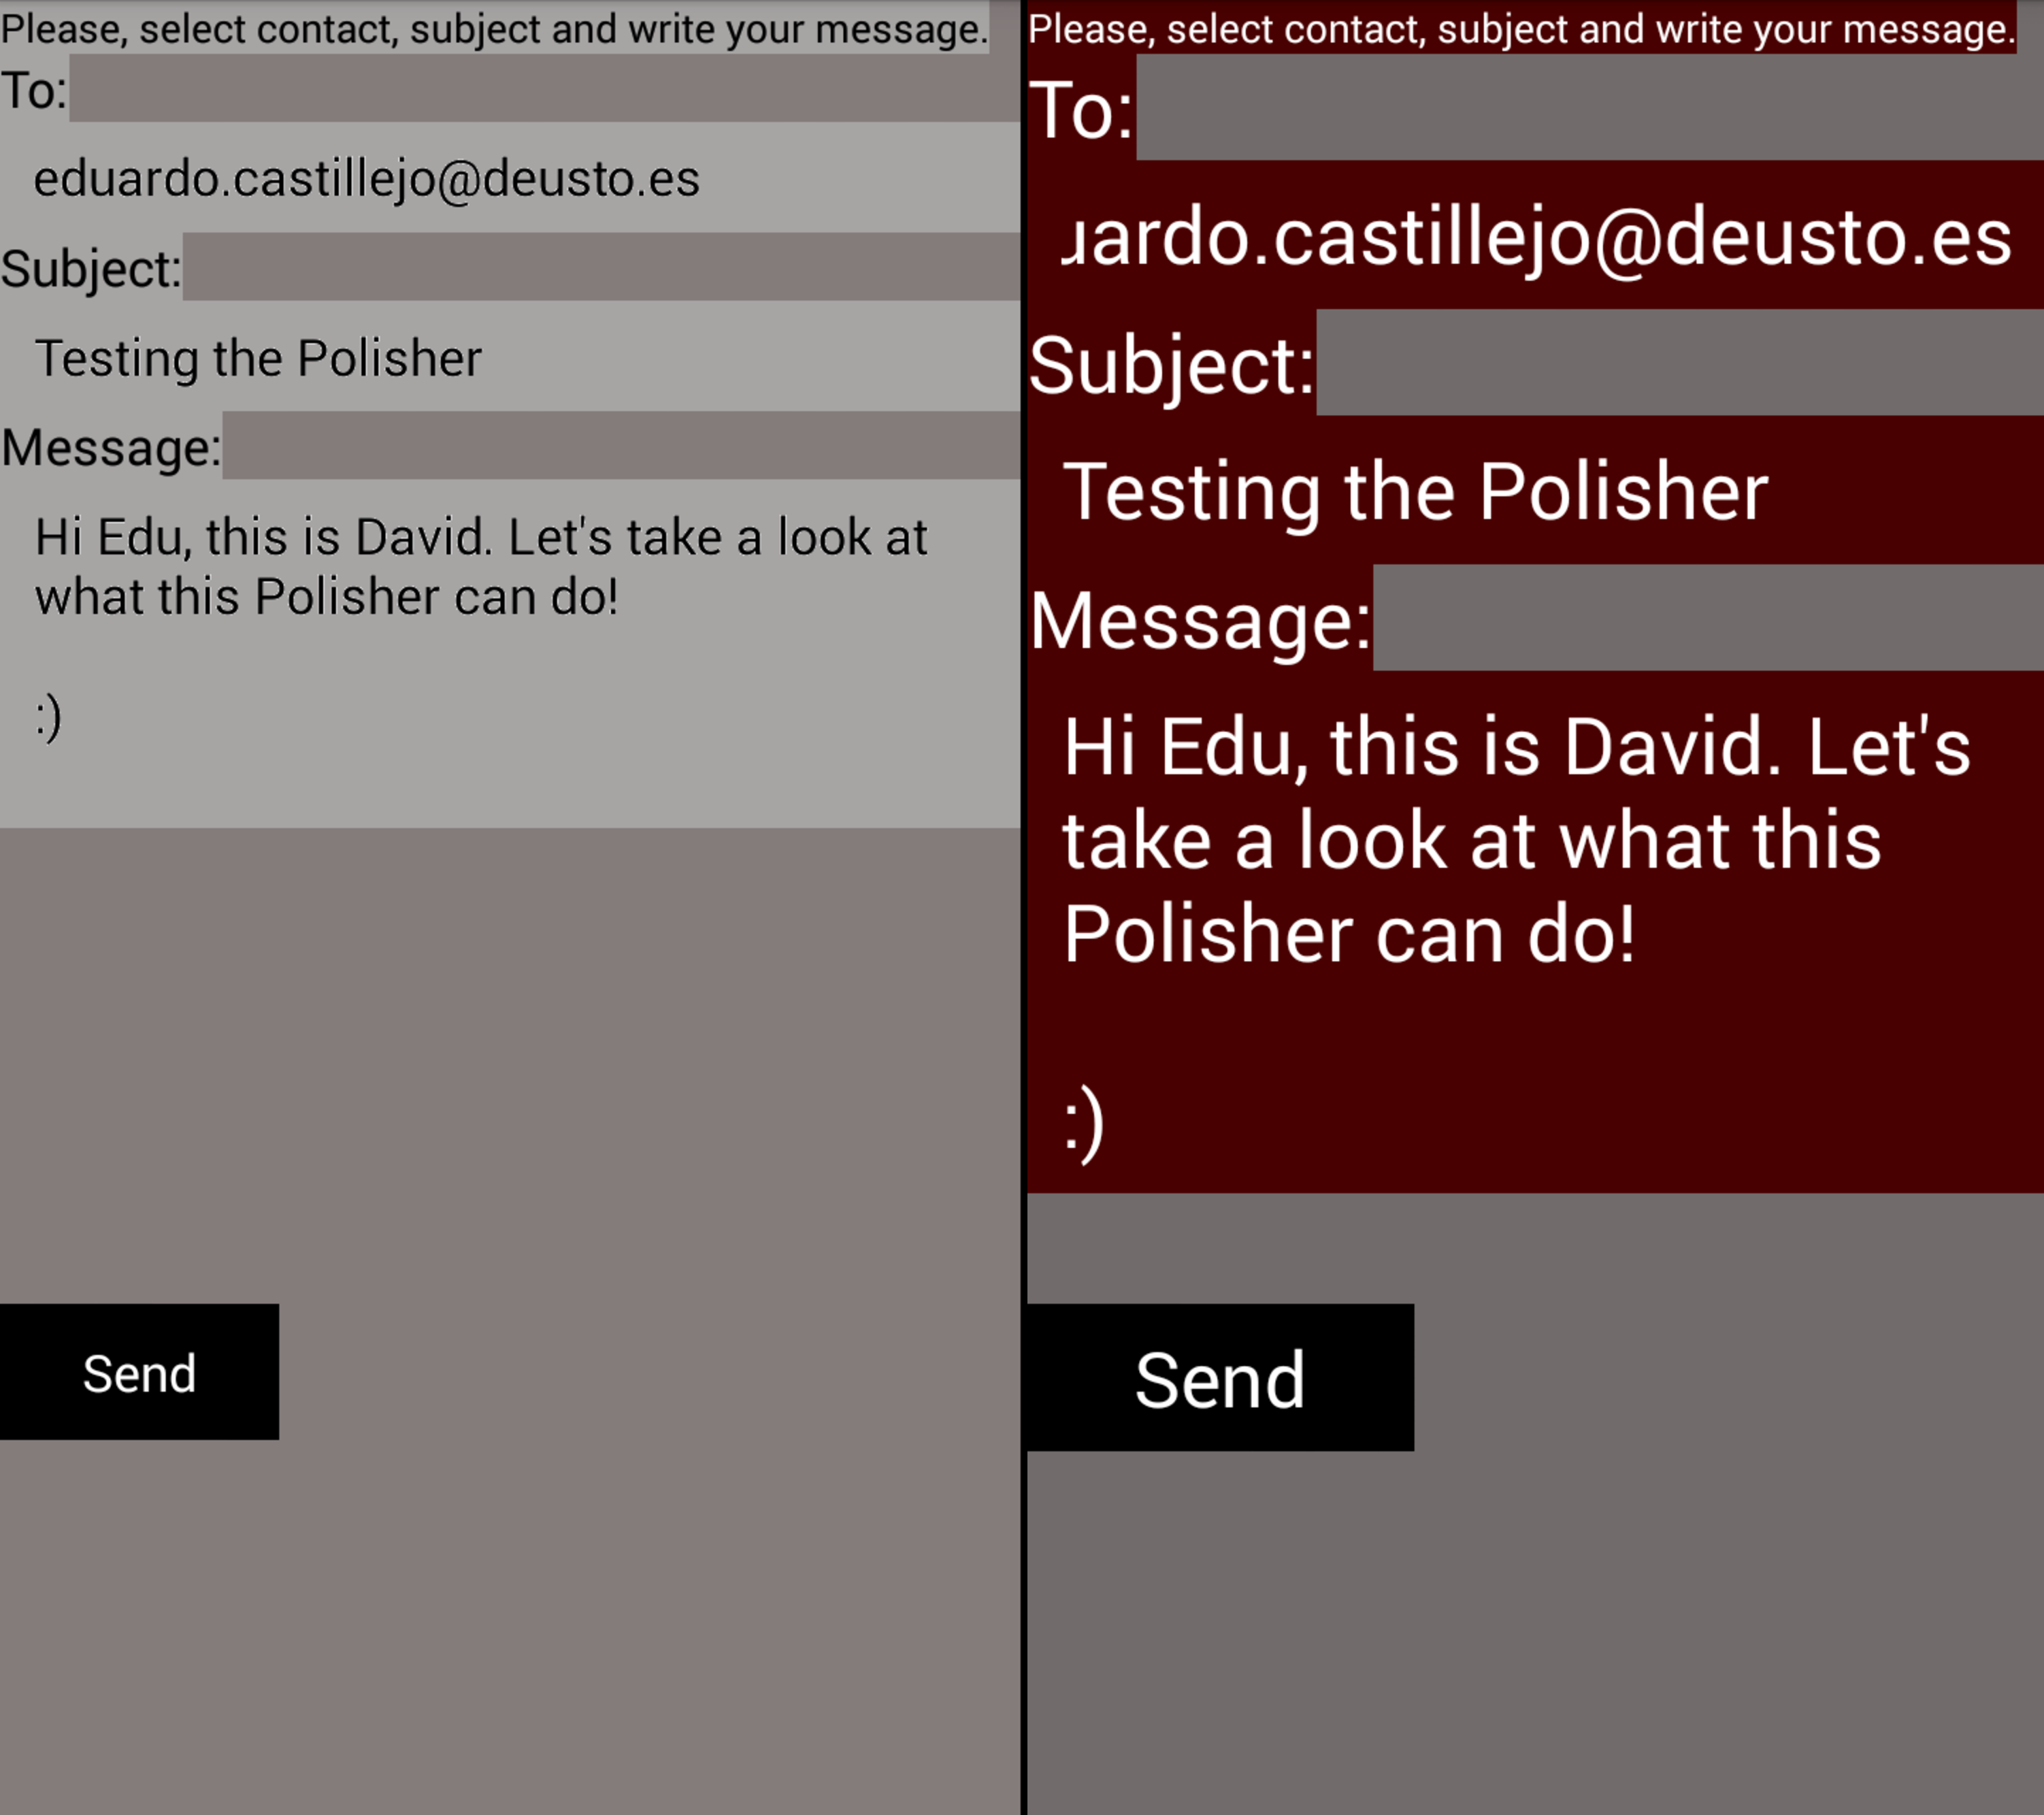
\includegraphics[width=0.65\textwidth]{polisher_4.pdf}
\caption{Polished user interface. On the left, the adapted version. On the 
right, the polished one.}
\label{fig:polisher_4}
\end{figure}